\documentclass[a4paper]{article}

\usepackage{amsmath}
\usepackage[english]{babel}
\usepackage[babel=true]{microtype}
\usepackage{wrapfig}
\usepackage{url}
\usepackage{mathrsfs} 
\usepackage[absolute]{textpos}
\usepackage{graphicx}
\usepackage{geometry}
\geometry{a4paper,left=40mm,right=30mm, top=3cm, bottom=3cm} 
\usepackage{subcaption}
\usepackage{float}

\newcommand{\Fermi}{\textit{Fermi} }

\begin{document}

\begin{figure}[t]
	\centering
	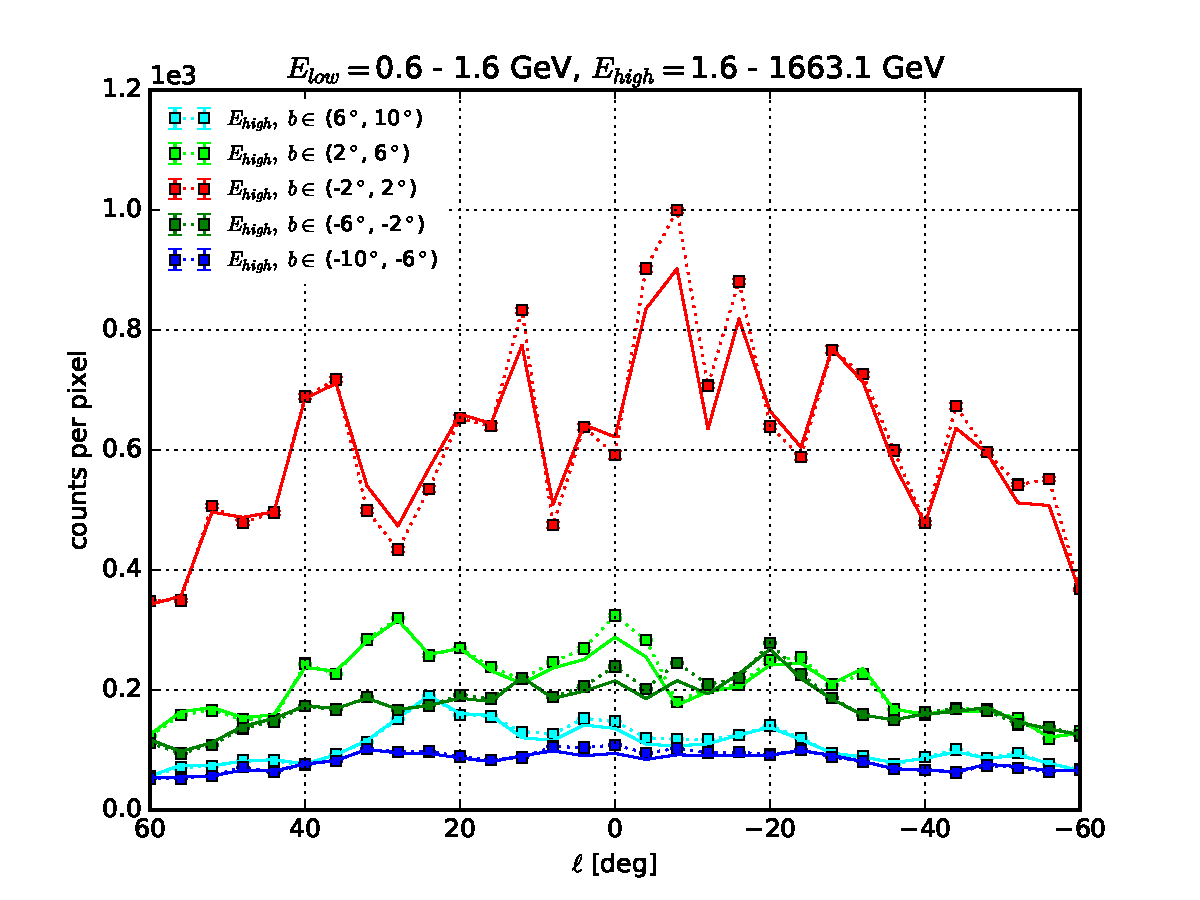
\includegraphics[width=0.7\textwidth]{FitE_profile_plot_at_0-1_to_1-1663.pdf}
    \caption{Longitudinal profiles of photon counts per pixel at small latitudes. Darker colours indicate latitude stripes above the Galactic plane, lighter colours indicate latitude stripes below. The region of the bubbles, i.e., $\ell \in (-20^\circ,20^\circ)$, is excluded from the fit. Point sources are masked.}
    \label{lowE_likelihood_profiles}
\end{figure}



\begin{figure}[H]
	\makebox[\linewidth][c]{%
	\begin{subfigure}[b]{.5\textwidth}
		\centering
		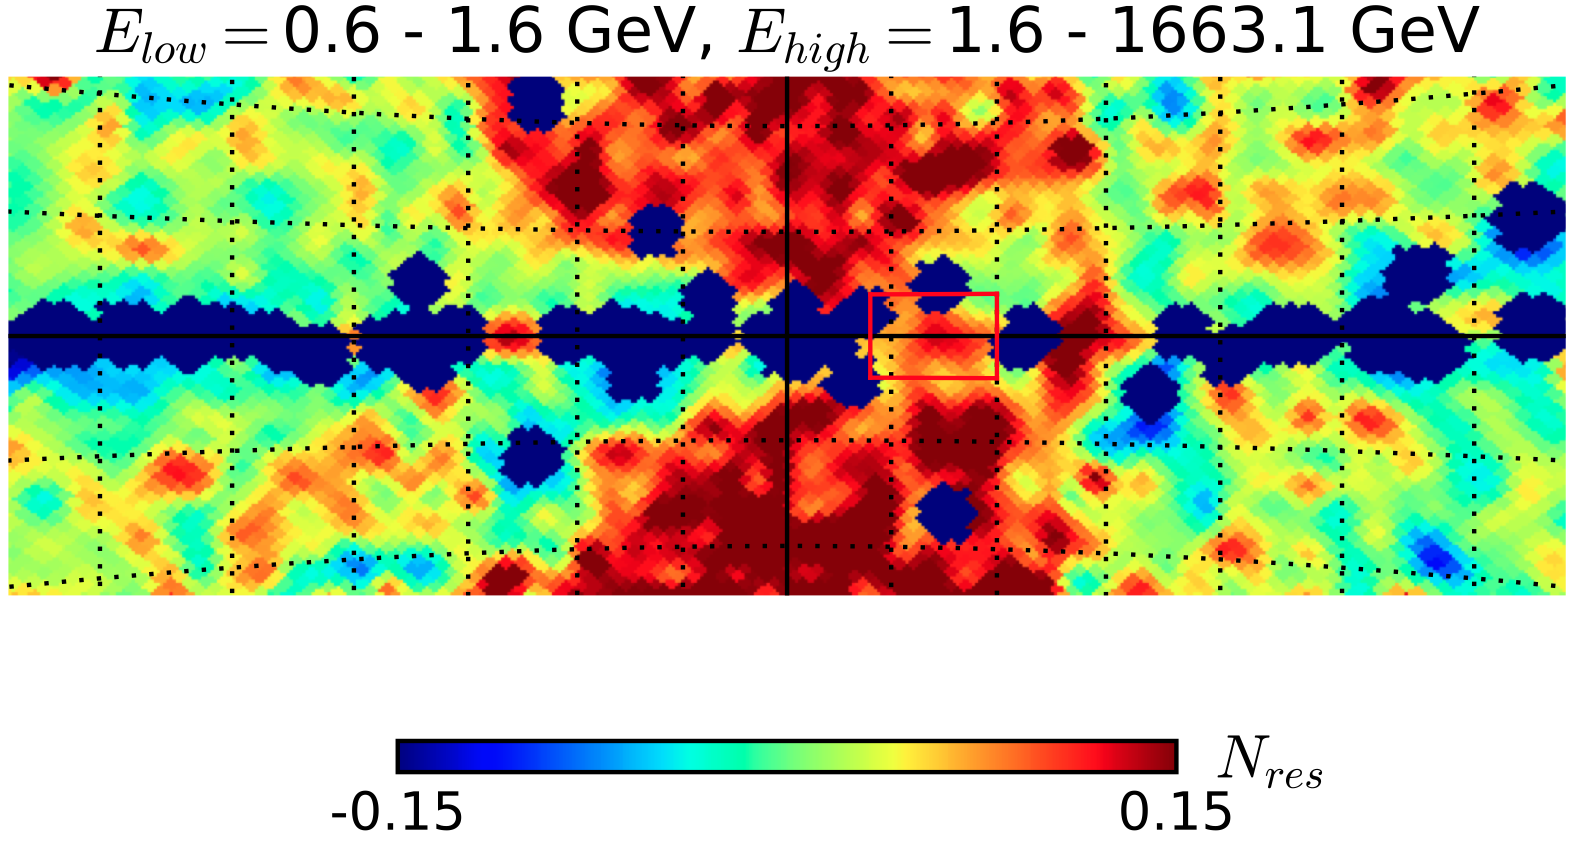
\includegraphics[width=.95\textwidth]{gnomview}
		\vspace*{1cm}
	\end{subfigure}%
	\begin{subfigure}[b]{.5\textwidth}
		\centering
		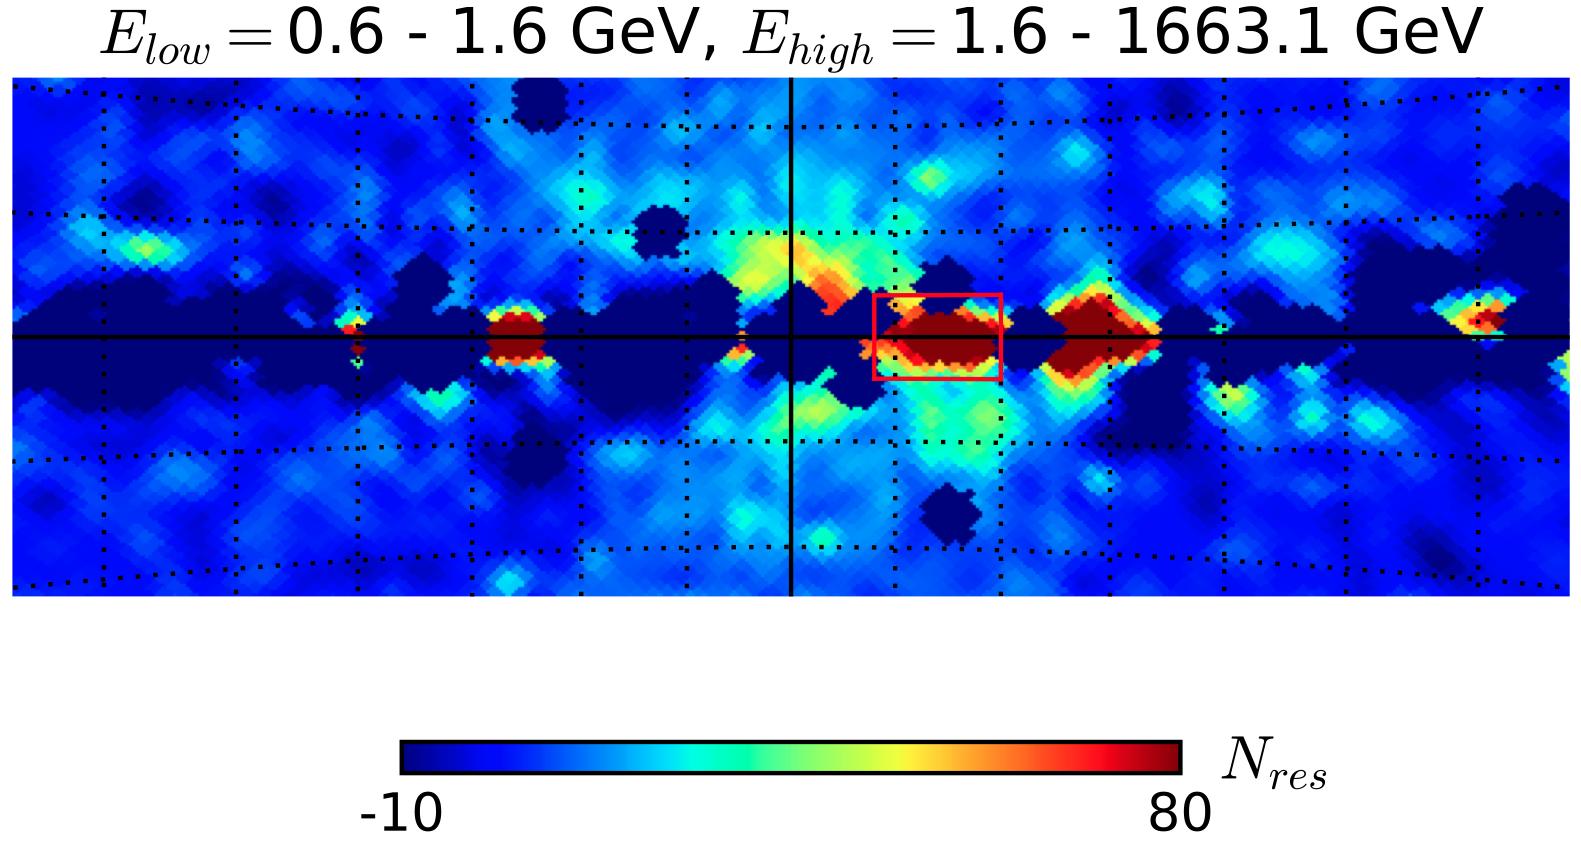
\includegraphics[width=.95\textwidth]{gnomview_nonorm}
		\vspace*{1cm}
	\end{subfigure}%
	}\\
	\vspace*{1cm}
	\makebox[\linewidth][c]{%
	\begin{subfigure}[b]{.5\textwidth}
		\centering
		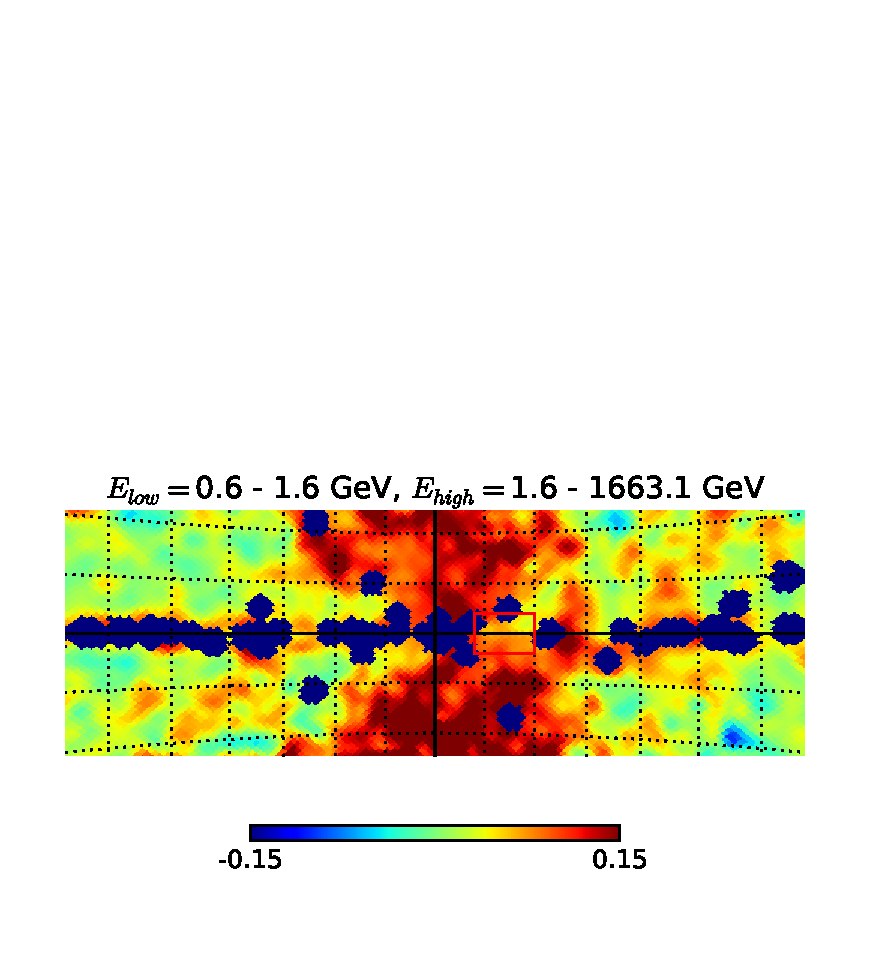
\includegraphics[width=.95\textwidth]{gnomview_highEsmooth}
	\end{subfigure}%
	\begin{subfigure}[b]{.5\textwidth}
		\centering
		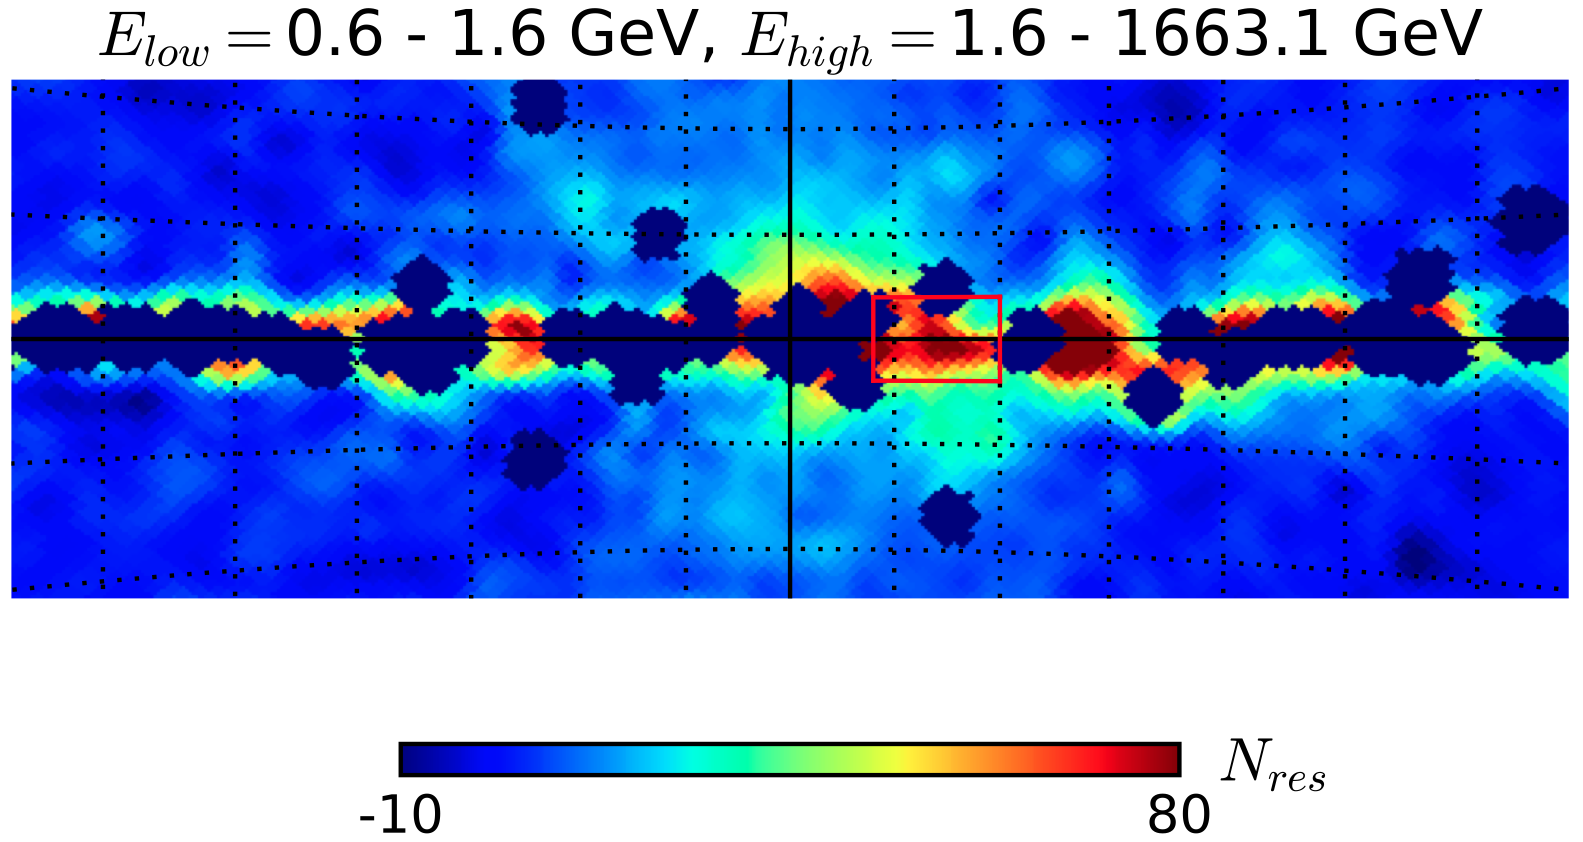
\includegraphics[width=.95\textwidth]{gnomview_highEsmooth_nonorm}
	\end{subfigure}%
	}\\
		\makebox[\linewidth][c]{%
	\begin{subfigure}[b]{.5\textwidth}
		\centering
		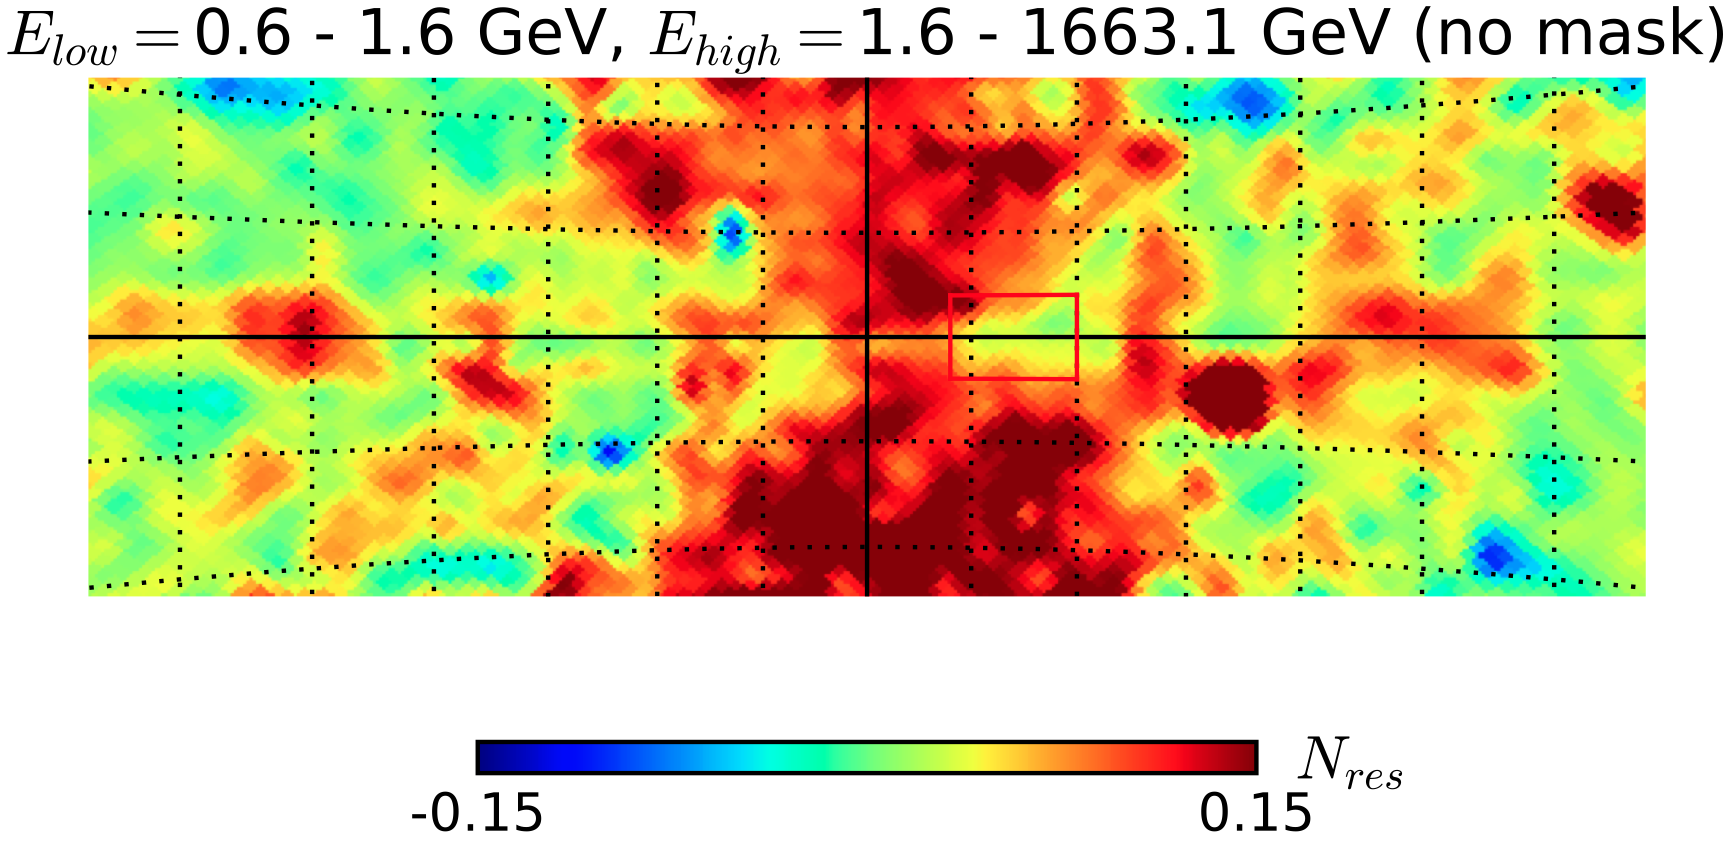
\includegraphics[width=.95\textwidth]{gnomview_highEsmooth_nomask}
	\end{subfigure}%
	\begin{subfigure}[b]{.5\textwidth}
		\centering
		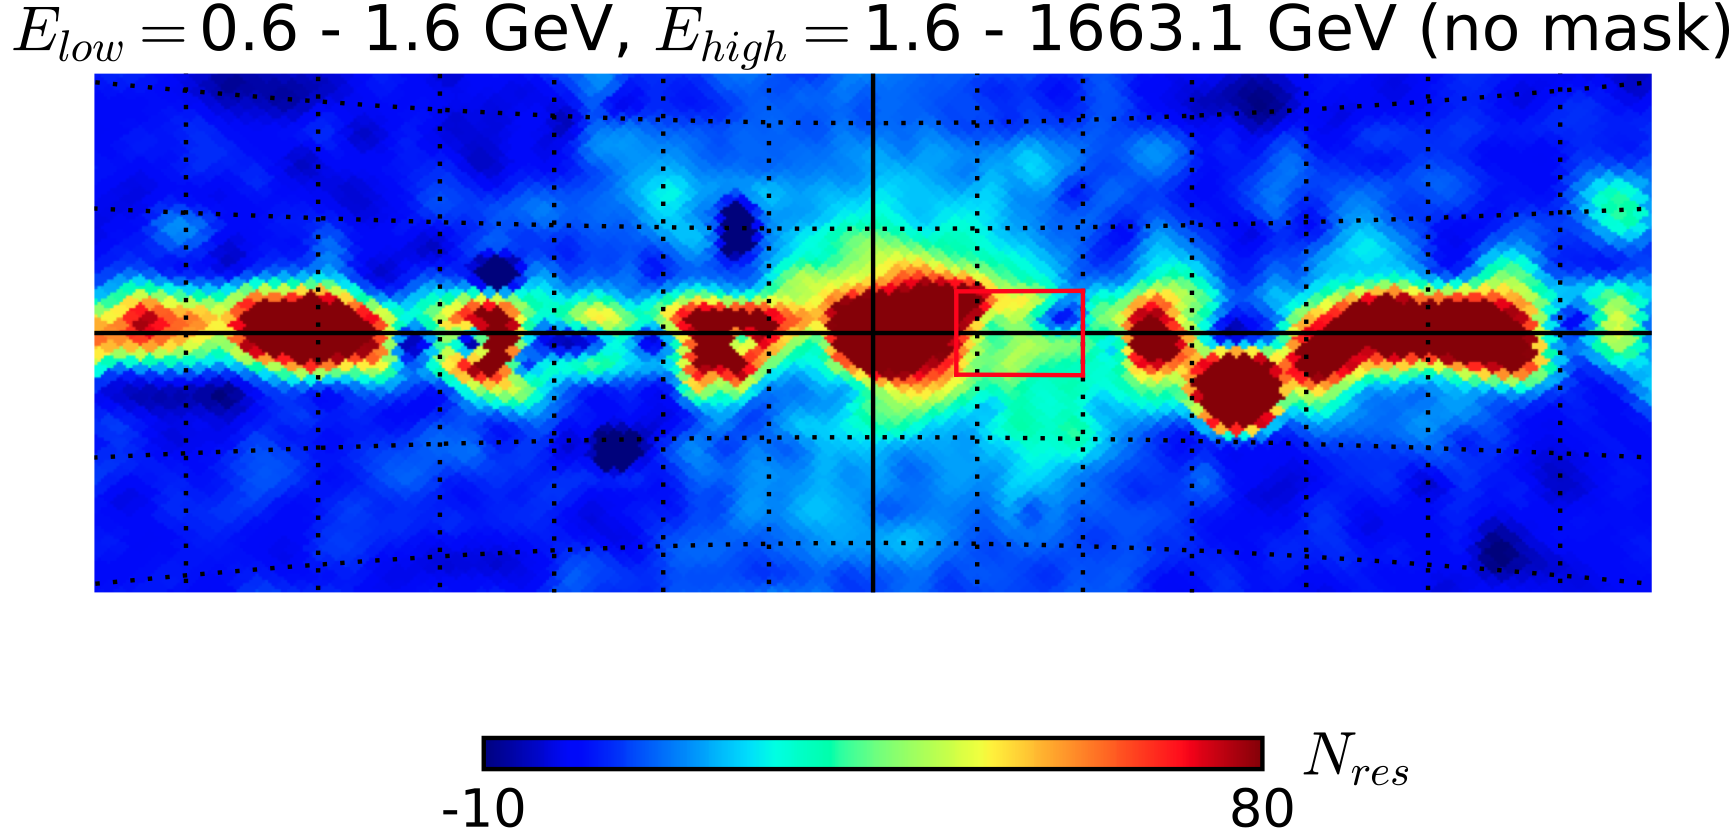
\includegraphics[width=.95\textwidth]{gnomview_highEsmooth_nonorm_nomask}
	\end{subfigure}%
	}\\
\caption{Residual photon-counts maps of the Galactic plane normalized (left) and not normalized (right). \textit{First row:} Point sources are masked and shown as the minimum value of the scale (dark blue). \textit{Second row:} The high-energy data is smoothed with a $0.5^\circ$ sigma Gaussian. \textit{Third row:} Point sources are not masked, high-energy data is smoothed. In order to avoid artefacts in the maps without mask resulting from the high fluxes of two very bright point sources on the western hemisphere (one is Crab nebula), the likelihood fit does not take into account the longitudes 0-$90^\circ$. The distance between two graticules is $5^\circ$}
\label{Fit_IC_pi0_to_ROI}
\end{figure}



\begin{figure}[h!]
	\makebox[\linewidth][c]{%
	\begin{subfigure}[b]{.5\textwidth}
		\centering
		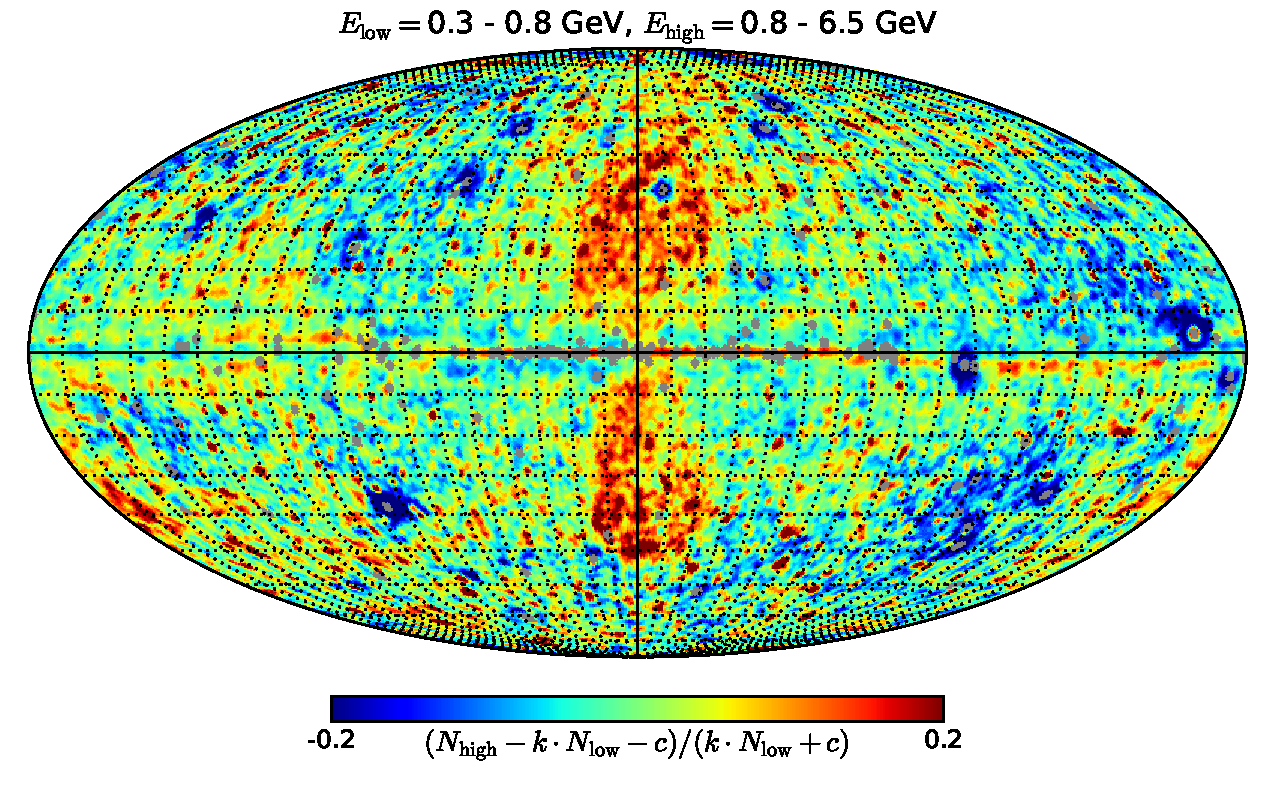
\includegraphics[width=.95\textwidth]{FitE_mollweide_at_0-0_to_0-6_norm02.pdf}
	\end{subfigure}%
	\begin{subfigure}[b]{.5\textwidth}
		\centering
		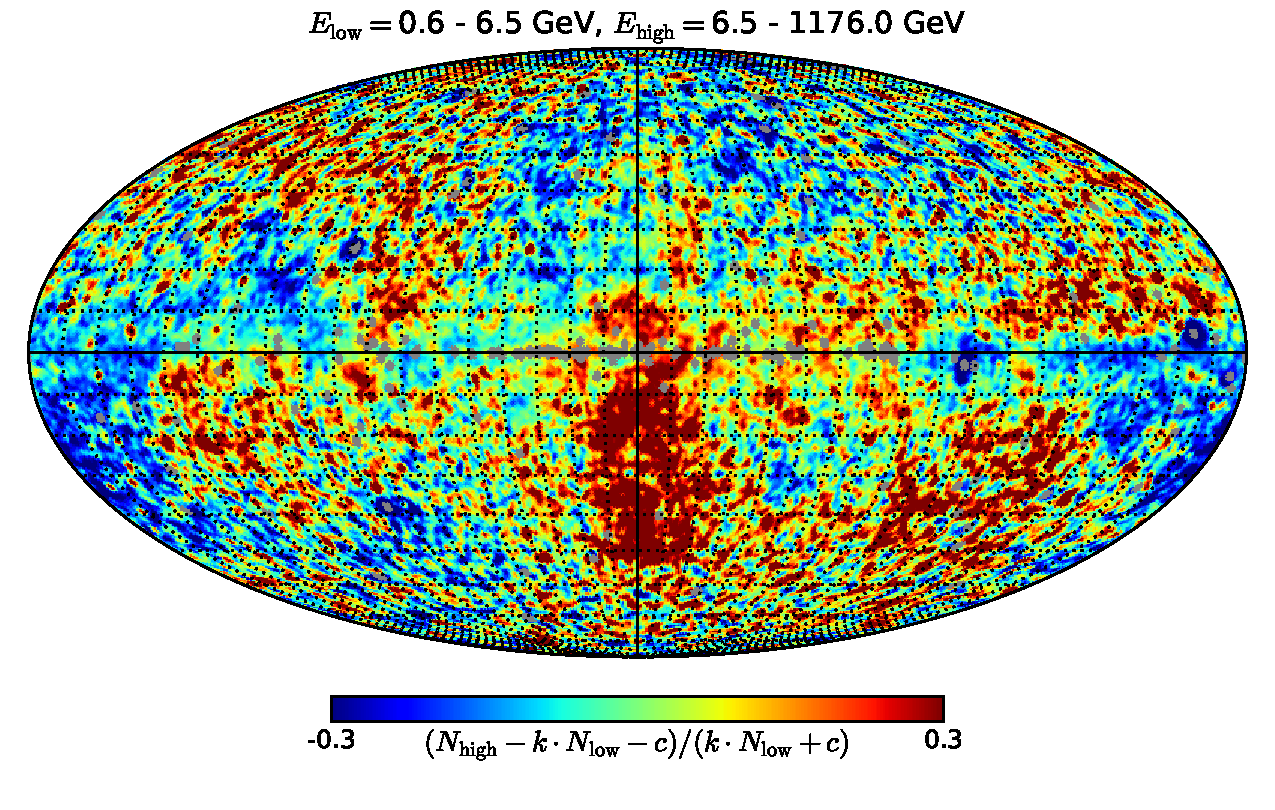
\includegraphics[width=.95\textwidth]{FitE_mollweide_at_0-6_to_6-1175_norm03.pdf}
	\end{subfigure}%
	}\\
	\makebox[\linewidth][c]{%
	\begin{subfigure}[b]{.5\textwidth}
		\centering
		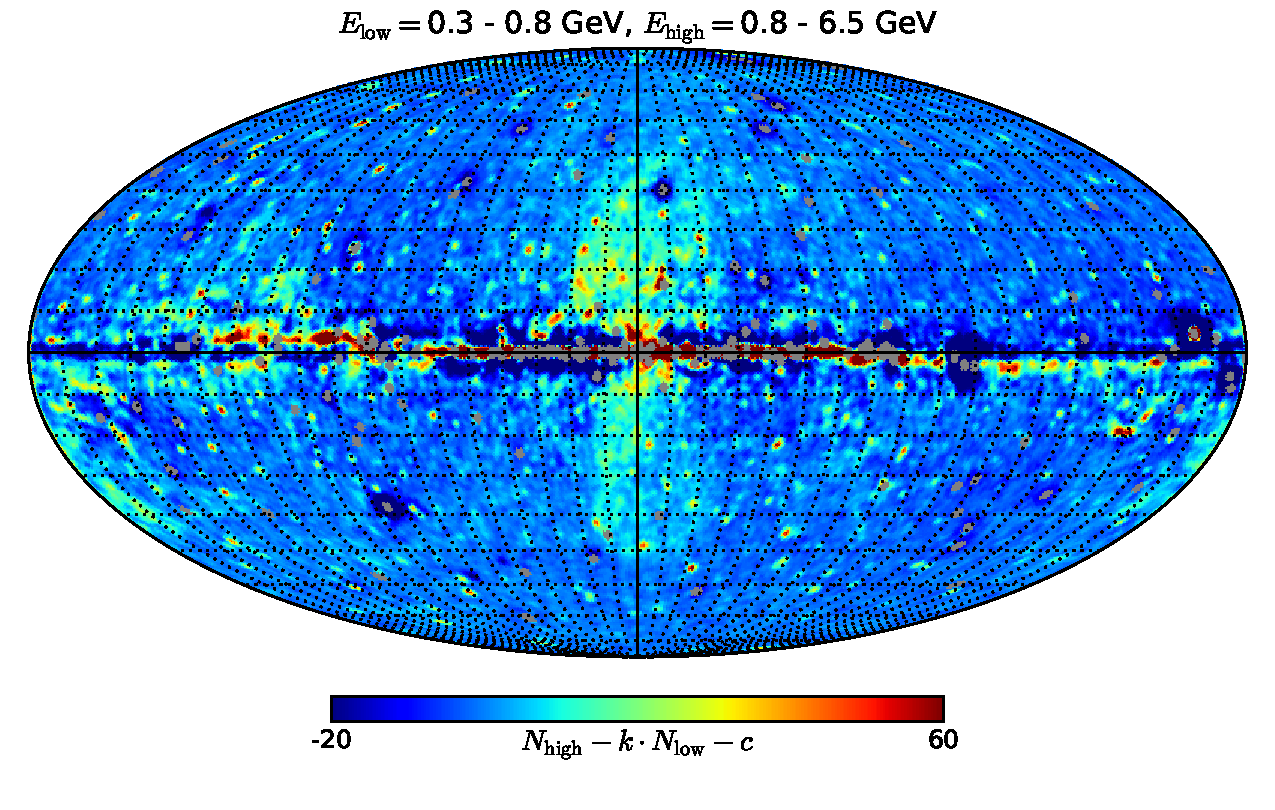
\includegraphics[width=.95\textwidth]{FitE_mollweide_at_0-0_to_0-6.pdf}
	\end{subfigure}%
	\begin{subfigure}[b]{.5\textwidth}
		\centering
		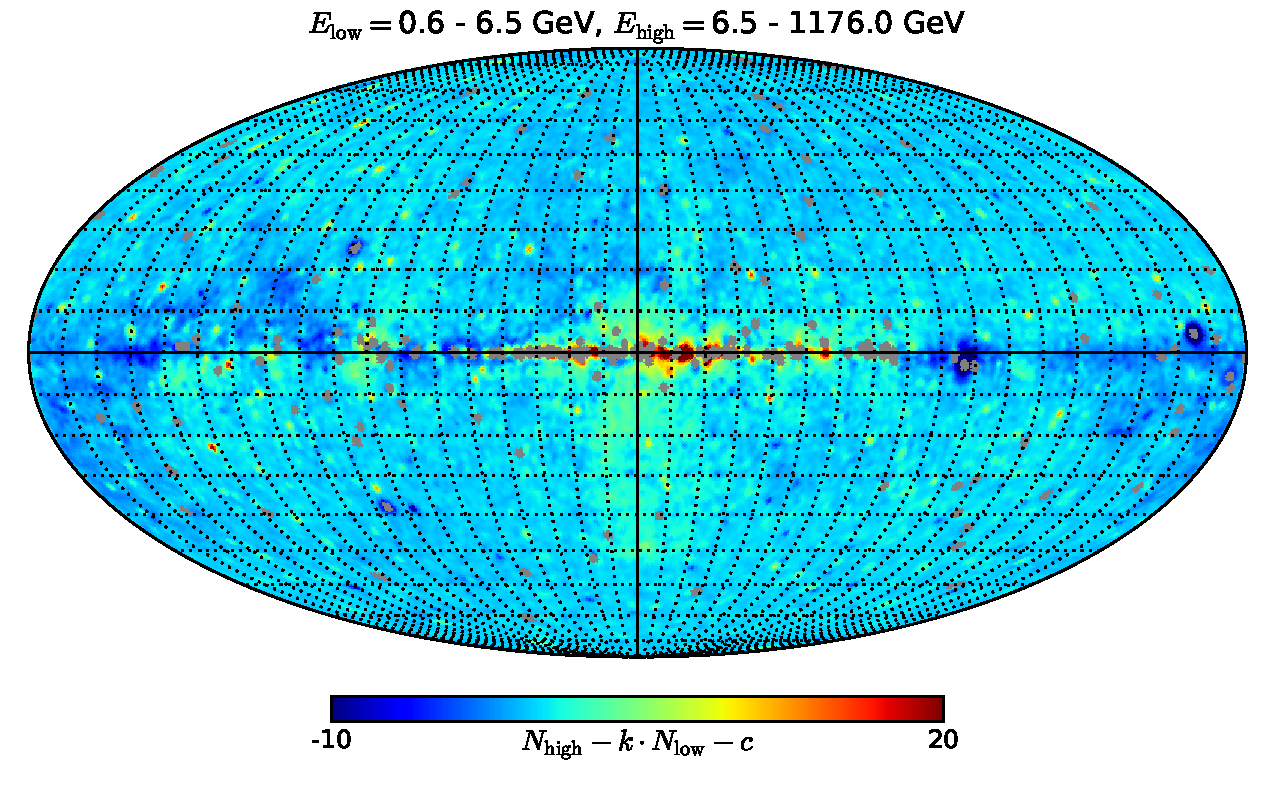
\includegraphics[width=.95\textwidth]{FitE_mollweide_at_0-6_to_6-1175.pdf}
	\end{subfigure}%
	}\\
\caption{Residual photon-counts map after subtraction of the model, normalized (left) and not normalized by the model (right). The energy range of the model is given by $E_{\text{high}}$, the energy range of the data by $E_{\text{low}}$. The map is smoothed with a Gaussian of $5^\circ$ FWHM. Point sources are masked.}
\label{Fit_IC_pi0_to_ROI}
\end{figure}




\begin{figure}[H]
	\makebox[\linewidth][c]{%
	\begin{subfigure}[b]{.5\textwidth}
		\centering
		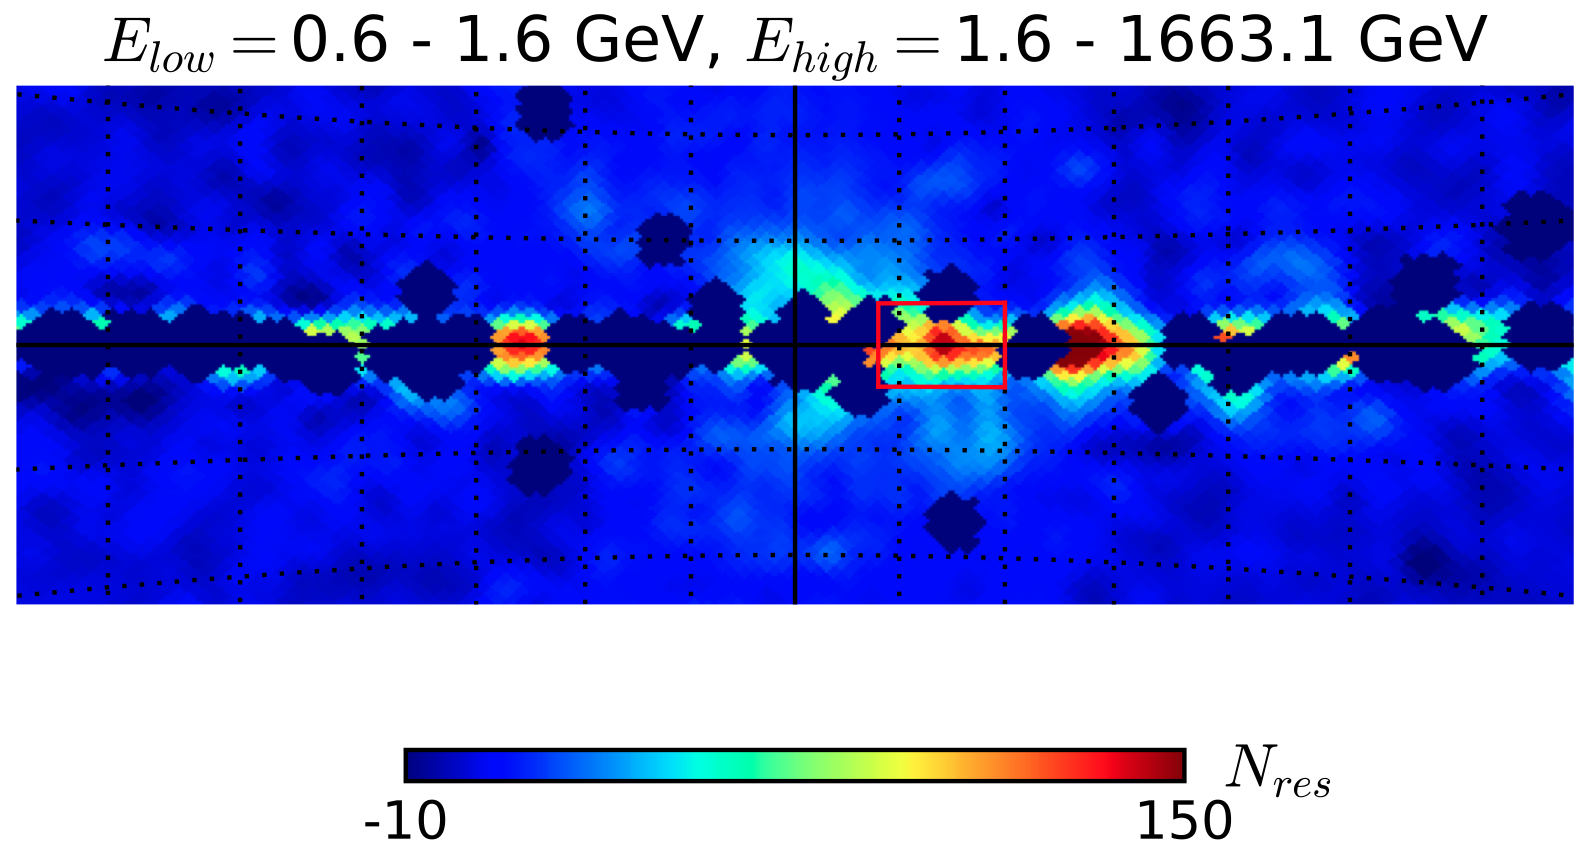
\includegraphics[width=.95\textwidth]{FitE_gnomview_at_0-1_to_1-1663_4deg}
		\vspace*{1cm}
	\end{subfigure}%
	\begin{subfigure}[b]{.5\textwidth}
		\centering
		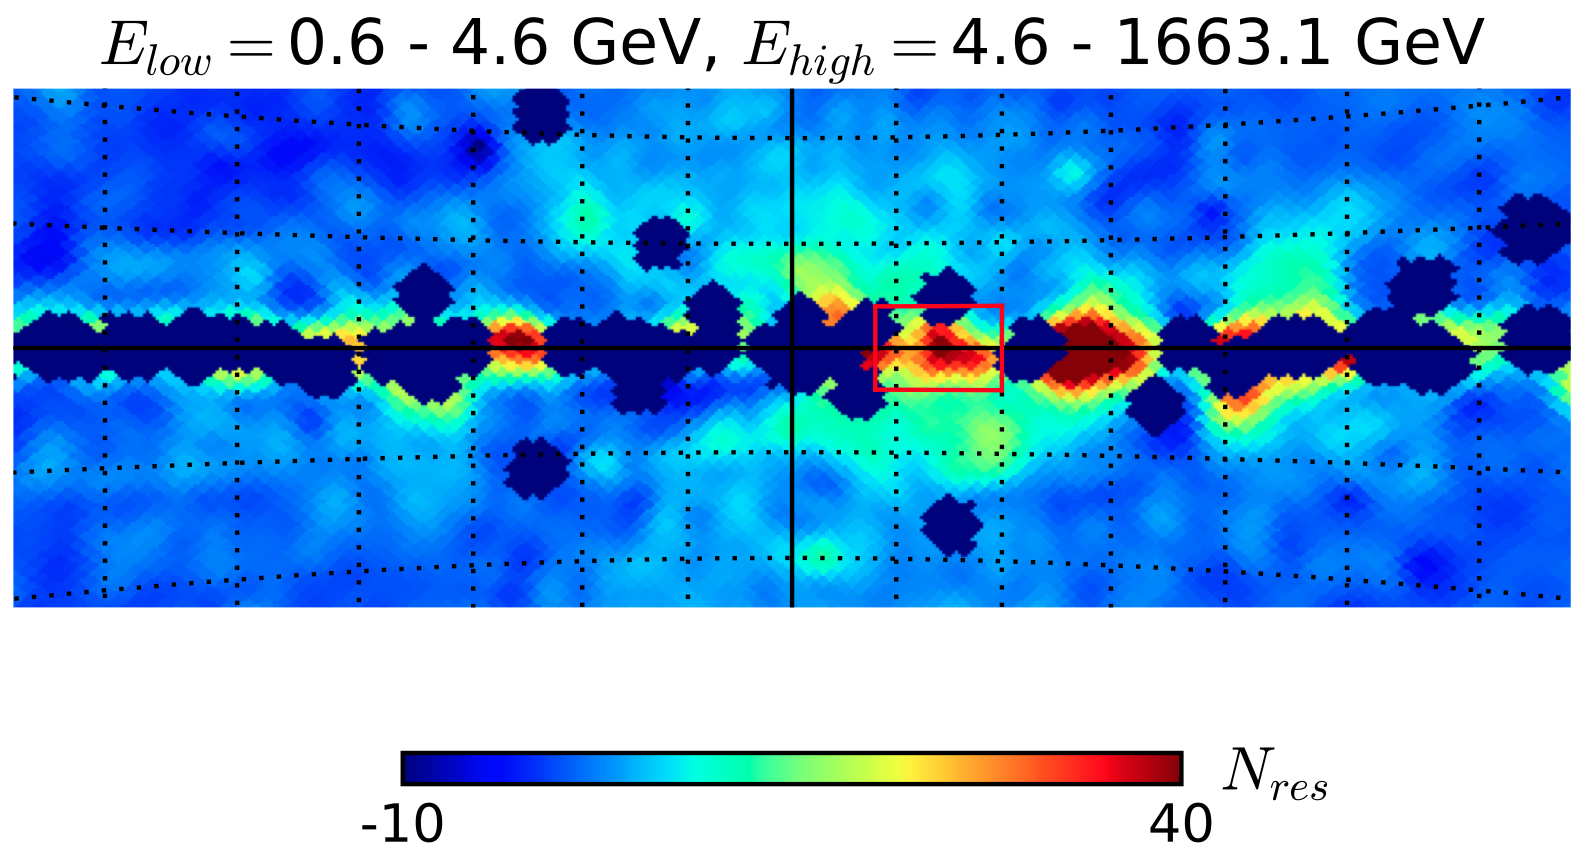
\includegraphics[width=.95\textwidth]{FitE_gnomview_at_0-4_to_4-1663_4deg}
		\vspace*{1cm}
	\end{subfigure}%
	}\\
	\makebox[\linewidth][c]{%
	\begin{subfigure}[b]{.5\textwidth}
		\centering
		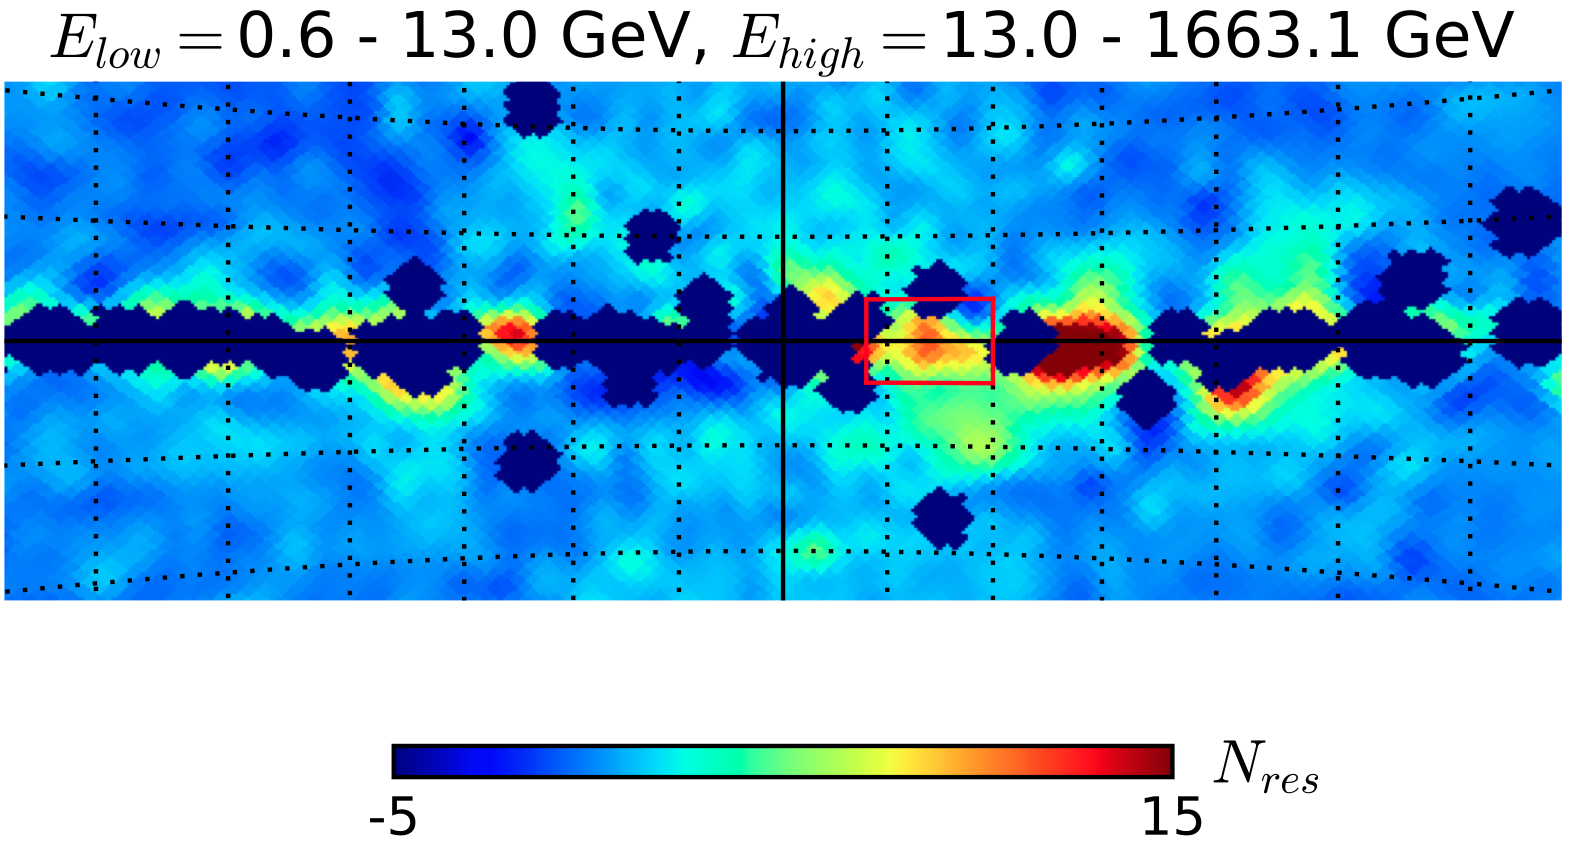
\includegraphics[width=.95\textwidth]{FitE_gnomview_at_0-12_to_12-1663_4deg}
	\end{subfigure}%
	\begin{subfigure}[b]{.5\textwidth}
		\centering
		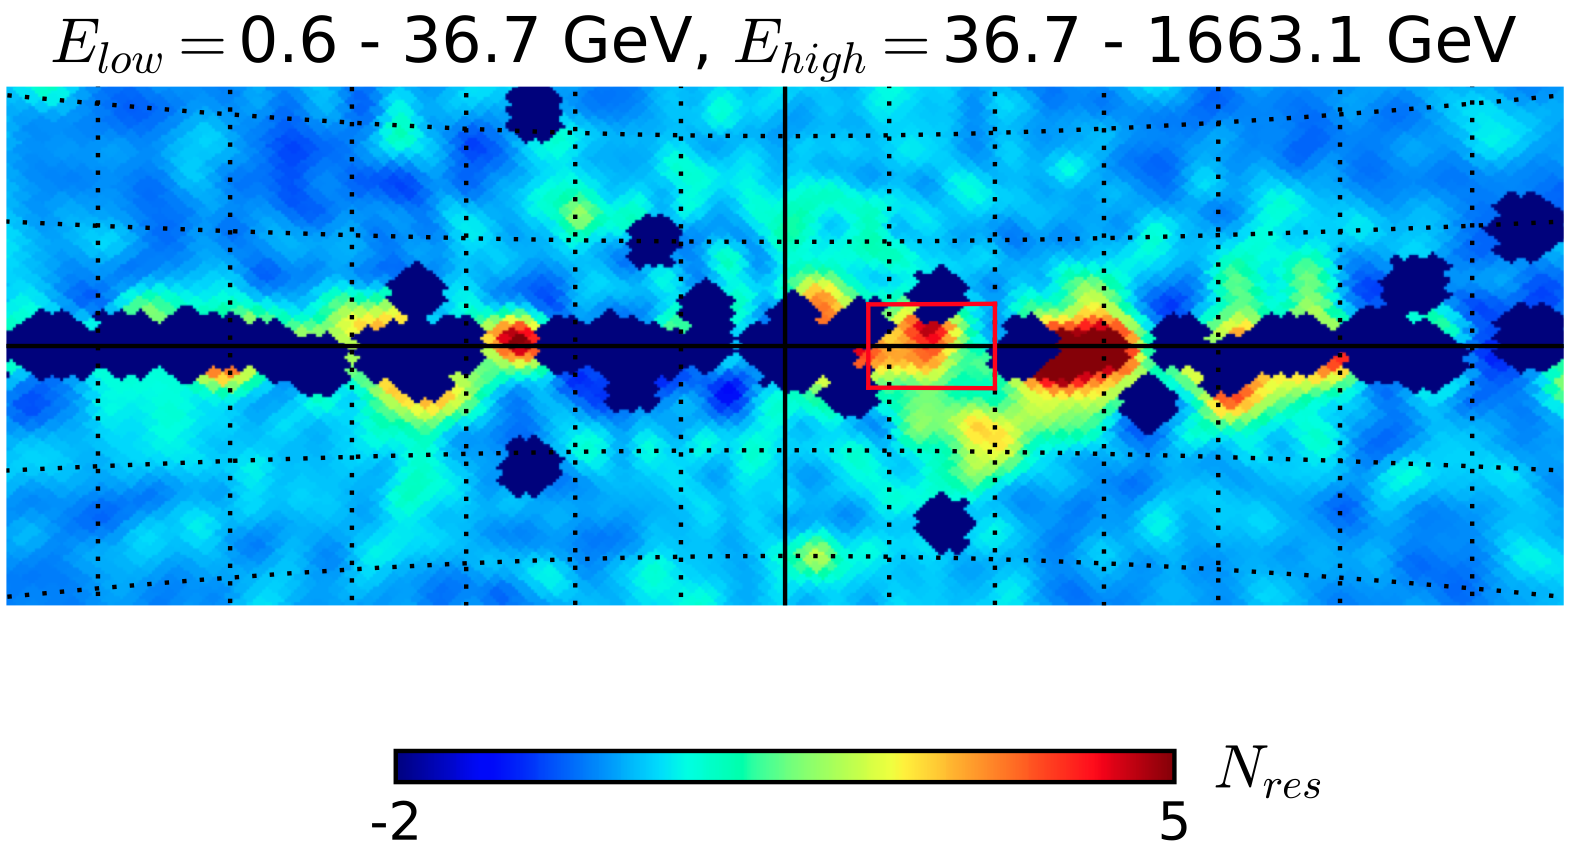
\includegraphics[width=.95\textwidth]{FitE_gnomview_at_0-36_to_36-1663_4deg}
	\end{subfigure}%
	}\\
\caption{Gnomview maps}
\label{Fit_IC_pi0_to_ROI}
\end{figure}



\end{document}
